\documentclass[]{book}
\usepackage{lmodern}
\usepackage{amssymb,amsmath}
\usepackage{ifxetex,ifluatex}
\usepackage{fixltx2e} % provides \textsubscript
\ifnum 0\ifxetex 1\fi\ifluatex 1\fi=0 % if pdftex
  \usepackage[T1]{fontenc}
  \usepackage[utf8]{inputenc}
\else % if luatex or xelatex
  \ifxetex
    \usepackage{mathspec}
  \else
    \usepackage{fontspec}
  \fi
  \defaultfontfeatures{Ligatures=TeX,Scale=MatchLowercase}
\fi
% use upquote if available, for straight quotes in verbatim environments
\IfFileExists{upquote.sty}{\usepackage{upquote}}{}
% use microtype if available
\IfFileExists{microtype.sty}{%
\usepackage{microtype}
\UseMicrotypeSet[protrusion]{basicmath} % disable protrusion for tt fonts
}{}
\usepackage{hyperref}
\hypersetup{unicode=true,
            pdftitle={High School Geometry},
            pdfauthor={Steven Allyn Taylor},
            pdfborder={0 0 0},
            breaklinks=true}
\urlstyle{same}  % don't use monospace font for urls
\usepackage{natbib}
\bibliographystyle{apalike}
\usepackage{longtable,booktabs}
\usepackage{graphicx,grffile}
\makeatletter
\def\maxwidth{\ifdim\Gin@nat@width>\linewidth\linewidth\else\Gin@nat@width\fi}
\def\maxheight{\ifdim\Gin@nat@height>\textheight\textheight\else\Gin@nat@height\fi}
\makeatother
% Scale images if necessary, so that they will not overflow the page
% margins by default, and it is still possible to overwrite the defaults
% using explicit options in \includegraphics[width, height, ...]{}
\setkeys{Gin}{width=\maxwidth,height=\maxheight,keepaspectratio}
\IfFileExists{parskip.sty}{%
\usepackage{parskip}
}{% else
\setlength{\parindent}{0pt}
\setlength{\parskip}{6pt plus 2pt minus 1pt}
}
\setlength{\emergencystretch}{3em}  % prevent overfull lines
\providecommand{\tightlist}{%
  \setlength{\itemsep}{0pt}\setlength{\parskip}{0pt}}
\setcounter{secnumdepth}{5}
% Redefines (sub)paragraphs to behave more like sections
\ifx\paragraph\undefined\else
\let\oldparagraph\paragraph
\renewcommand{\paragraph}[1]{\oldparagraph{#1}\mbox{}}
\fi
\ifx\subparagraph\undefined\else
\let\oldsubparagraph\subparagraph
\renewcommand{\subparagraph}[1]{\oldsubparagraph{#1}\mbox{}}
\fi

%%% Use protect on footnotes to avoid problems with footnotes in titles
\let\rmarkdownfootnote\footnote%
\def\footnote{\protect\rmarkdownfootnote}

%%% Change title format to be more compact
\usepackage{titling}

% Create subtitle command for use in maketitle
\providecommand{\subtitle}[1]{
  \posttitle{
    \begin{center}\large#1\end{center}
    }
}

\setlength{\droptitle}{-2em}

  \title{High School Geometry}
    \pretitle{\vspace{\droptitle}\centering\huge}
  \posttitle{\par}
    \author{Steven Allyn Taylor}
    \preauthor{\centering\large\emph}
  \postauthor{\par}
      \predate{\centering\large\emph}
  \postdate{\par}
    \date{2019: Last compiled 2019-06-17}

\usepackage{booktabs}
\usepackage{amsthm}
\makeatletter
\def\thm@space@setup{%
  \thm@preskip=8pt plus 2pt minus 4pt
  \thm@postskip=\thm@preskip
}
\makeatother

\begin{document}
\maketitle

{
\setcounter{tocdepth}{1}
\tableofcontents
}
\chapter*{Preface}\label{preface}
\addcontentsline{toc}{chapter}{Preface}

\begin{center}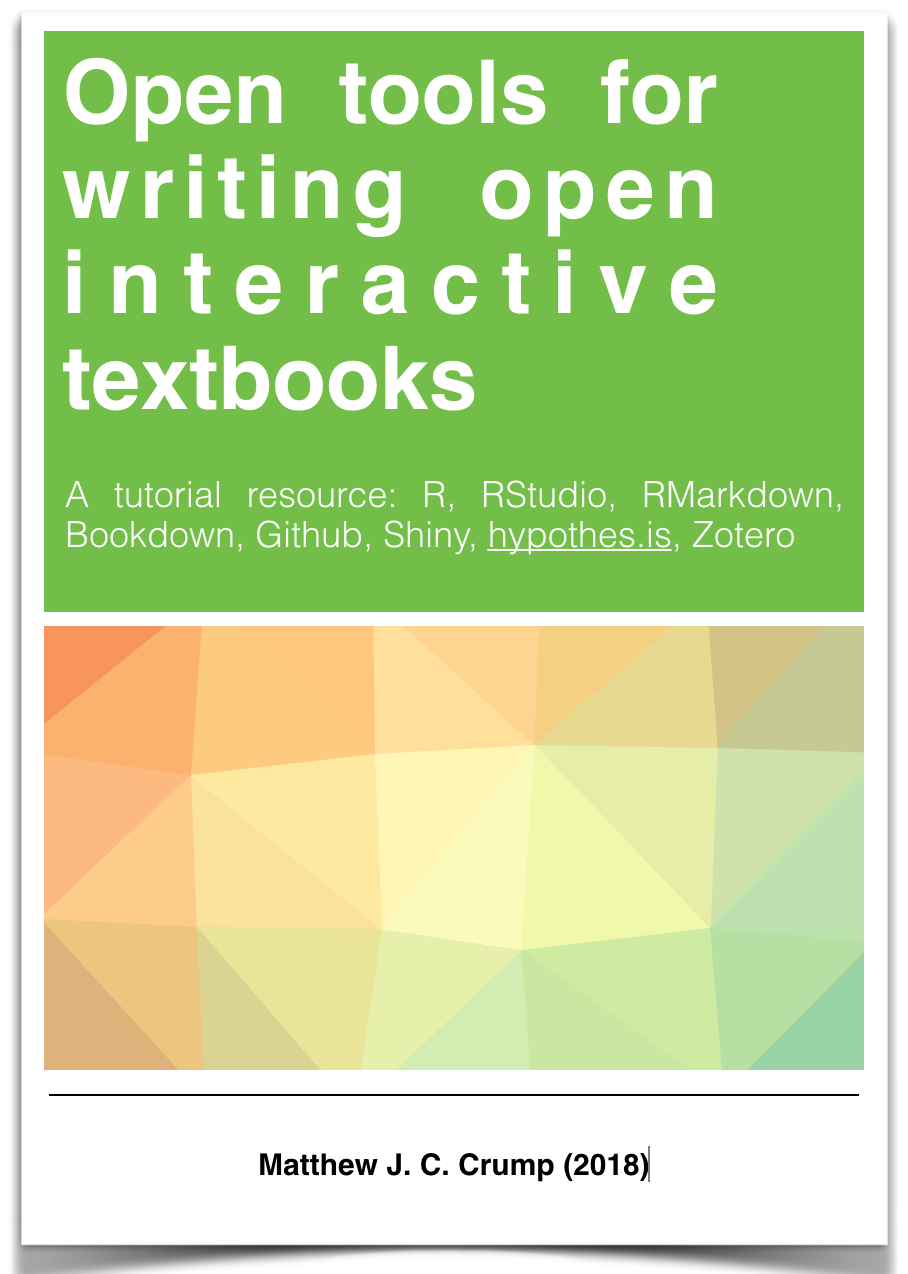
\includegraphics{OER} \end{center}

Taylor, Steven A. (2018). High School Geometry.
\url{https://phsmath.github.io/OERGeometry/}

This is an Open Education Resource for High School Geometry that meets
the requirements or Oregon's High School Math Standards.

This web-book is itself a work in progress. All of the source code
needed to compile this book yourself is included in the
\href{https://github.com/PHSMath/OERGeometry}{github repository for this
book}. You can download the repository, replace this text with your own,
and then compile your book as a web-page, .pdf or epub.

Feel free to note any typographical errors or other problems by
submitting an issue to this repository.

\textbf{License CC BY-SA 4.0 license}

The book is released under a creative commons
\href{https://creativecommons.org/licenses/by-sa/4.0/}{CC BY-SA 4.0}
license. This means that this book can be reused, remixed, retained,
revised and redistributed (including commercially) as long as
appropriate credit is given to the authors. If you remix, or modify the
original version of this open textbook, you must redistribute all
versions of this open textbook under the same license - CC BY-SA 4.0.

\chapter{Reasoning and Proof}\label{reasoning-and-proof}

\section{Axiomatic Development of
Mathematics}\label{axiomatic-development-of-mathematics}

\subsection{Undefined Terms}\label{undefined-terms}

\subsection{Undefined Relations}\label{undefined-relations}

\subsection{Axioms Relating the Undefined Terms and Undefined
Relations}\label{axioms-relating-the-undefined-terms-and-undefined-relations}

\subsection{Theorems}\label{theorems}

\section{Logic and Propositional
Calculus}\label{logic-and-propositional-calculus}

\subsection{Propositions and Compound
Propositions}\label{propositions-and-compound-propositions}

\section{Reasoning}\label{reasoning}

\subsection{Inductive Reasoning}\label{inductive-reasoning}

\subsection{Deductive Reasoning}\label{deductive-reasoning}

\section{Logical Operations}\label{logical-operations}

\subsection{Conditional Statements}\label{conditional-statements}

\subsection{Basic Logical Operations}\label{basic-logical-operations}

\subsection{Propositions and Truth
Tables}\label{propositions-and-truth-tables}

\subsection{Tautologies and
Contradictions}\label{tautologies-and-contradictions}

\subsection{Logical Equivalence}\label{logical-equivalence}

\subsection{Algebra of Propositions}\label{algebra-of-propositions}

\subsection{Conditional and Biconditional
Statements}\label{conditional-and-biconditional-statements}

\subsection{Arguments}\label{arguments}

\subsection{Logical Implication}\label{logical-implication}

\section{Sets and Basic Operations on
Sets}\label{sets-and-basic-operations-on-sets}

\subsection{Introduction}\label{introduction}

\subsection{Sets and Elements}\label{sets-and-elements}

\subsection{Universal Set, Empty Set}\label{universal-set-empty-set}

\subsection{Subsets}\label{subsets}

\subsection{Venn Diagrams}\label{venn-diagrams}

\subsection{Set Operations}\label{set-operations}

\subsection{Algebra of Sets}\label{algebra-of-sets}

\subsection{Finite Sets, Counting
Principles}\label{finite-sets-counting-principles}

\subsection{Classes of Sets, Power
Sets}\label{classes-of-sets-power-sets}

\subsection{Arguments and Venn
Diagrams}\label{arguments-and-venn-diagrams}

\section{Reason Using Properties of
Algebra}\label{reason-using-properties-of-algebra}

\chapter{Essentials of Geometry}\label{essentials-of-geometry}

\section{Points, Lines, and Planes}\label{points-lines-and-planes}

\section{Segments and Congruence}\label{segments-and-congruence}

\section{Midpoint and Distance
Formulas}\label{midpoint-and-distance-formulas}

\section{Angles}\label{angles}

\section{Angle Pair Relationships}\label{angle-pair-relationships}

\section{Polygons}\label{polygons}

\section{Prove Statements About Segments and
Angles}\label{prove-statements-about-segments-and-angles}

\section{Prove Angle Pair
Relationshiops}\label{prove-angle-pair-relationshiops}

\chapter{Lines}\label{lines}

\section{Line and Angle Pairs}\label{line-and-angle-pairs}

\section{Parallel Lines and
Transversals}\label{parallel-lines-and-transversals}

\section{Slopes of Lines}\label{slopes-of-lines}

\section{Write and Graph Equations of
Lines}\label{write-and-graph-equations-of-lines}

\section{Perpendicular Lines}\label{perpendicular-lines}

\section{Intersection of Lines}\label{intersection-of-lines}

\chapter{Congruent Triangles}\label{congruent-triangles}

\section{Triangle Properties}\label{triangle-properties}

\subsection{Classification}\label{classification}

\subsection{Triangle Sum Theorem}\label{triangle-sum-theorem}

\subsection{Exterior Angle Theorem}\label{exterior-angle-theorem}

\section{Apply Congruence in
Triangles}\label{apply-congruence-in-triangles}

\subsection{Definitions}\label{definitions}

\subsection{Third Angles Theorem}\label{third-angles-theorem}

\subsection{Properties of Congruent
Triangles}\label{properties-of-congruent-triangles}

\section{Transformations and
Congruence}\label{transformations-and-congruence}

\subsection{Rigid Transformations}\label{rigid-transformations}

\subsubsection{Translation}\label{translation}

\subsubsection{Reflections}\label{reflections}

\subsubsection{Rotations}\label{rotations}

\subsection{Non-Rigid Transformations}\label{non-rigid-transformations}

\subsubsection{Dilations}\label{dilations}

\subsection{Perform Congruence
Transformations}\label{perform-congruence-transformations}

\subsubsection{Coordinate Notation}\label{coordinate-notation}

\subsubsection{Matrix and Vector
Notation}\label{matrix-and-vector-notation}

\subsection{Perform Non-Congruence
Transformations}\label{perform-non-congruence-transformations}

\subsubsection{Scalar Multiplation}\label{scalar-multiplation}

\section{Proving Triangles are
Congruent}\label{proving-triangles-are-congruent}

\subsection{Side-Side-Side Congruence
Postulate}\label{side-side-side-congruence-postulate}

\subsection{Side-Angle-Side Congruence
Postulate}\label{side-angle-side-congruence-postulate}

\subsection{Hypotenuse-Leg Congruence
Theorem}\label{hypotenuse-leg-congruence-theorem}

\subsection{Angle-Side-Angle Congruence
Theorem}\label{angle-side-angle-congruence-theorem}

\subsection{Angle-Angle-Side Congruence
Theorem}\label{angle-angle-side-congruence-theorem}

\section{Isoceles and Equilateral
Triangles}\label{isoceles-and-equilateral-triangles}

\subsection{Isosceles Triangles}\label{isosceles-triangles}

\subsubsection{Base Angles Theorem}\label{base-angles-theorem}

\subsubsection{Converse of Base Angles
Theorem}\label{converse-of-base-angles-theorem}

\subsection{Equilateral Triangles}\label{equilateral-triangles}

\subsubsection{Corollary of the Base Angles
Theorem}\label{corollary-of-the-base-angles-theorem}

\subsubsection{Corollary to the Converse of Base Angles
Theorem}\label{corollary-to-the-converse-of-base-angles-theorem}

\chapter{Relationships within
Triangles}\label{relationships-within-triangles}

\chapter{Similarity}\label{similarity}

\chapter{Right Triangles and
Trigonometry}\label{right-triangles-and-trigonometry}

\chapter{Quadrilaterals}\label{quadrilaterals}

\chapter{Transformations}\label{transformations}

\chapter{Circles}\label{circles}

\chapter{Measurements}\label{measurements}

\chapter{Probability}\label{probability}

\bibliography{book.bib,packages.bib}


\end{document}
